% Written by Martin Pasquier

\subsubsection{Objectif du site web}

Le site web est une tâche secondaire du projet, mais il est tout de même important pour la communication et la promotion du jeu.
Il est essentiel pour permettre aux joueurs de découvrir le jeu, de suivre son développement et de le télécharger.
C'est l'outils central de la partie communication du projet, et il est donc important de le maintenir à jour avec les dernières informations sur le jeu.

\subsubsection{Développement}

Le site possède son propre dépôt de code source sur GitHub à l'adresse \url{https://github.com/StonksIndustries/Azerith_Website}.
Nous avons utilisé l'éditeur de code VSCode pour développer le site web car il offre de nombreux outils très utiles pour cela.
On peut citer l'intégration avec GitHub, les extensions pour le développement web, et les outils de débogage intégrés.
\\

Le site web est développé en HTML, SCSS et JS, et est compilé avec Parcel.
Leur choix a été motivé par leur simplicité et leur popularité, qui permettent de trouver facilement de l'aide en cas de problème.
Parcel permet de compiler le site web sans aucune configuration et une très bonne optimisation des fichiers générés.
Le SCSS, remplace le CSS pour permettre une meilleure organisation du code et une meilleure maintenabilité.
Le JS est utilisé pour les quelques animations et les interactions avec le visiteur.
\\

Il sera automatiquement compilé et publié grâce aux outils GitHub Actions et GitHub Pages.
L'usage de ces outils permet de simplifier la publication du site web, et de le mettre à jour automatiquement à chaque modification du code source.
Chaque nouvelle versions envoyés par un développeur est automatiquement compilée et publiée sur le site web si aucune erreur n'est détectée.

\subsubsection{Apparence}

\begin{figure}[H]
    \centering
    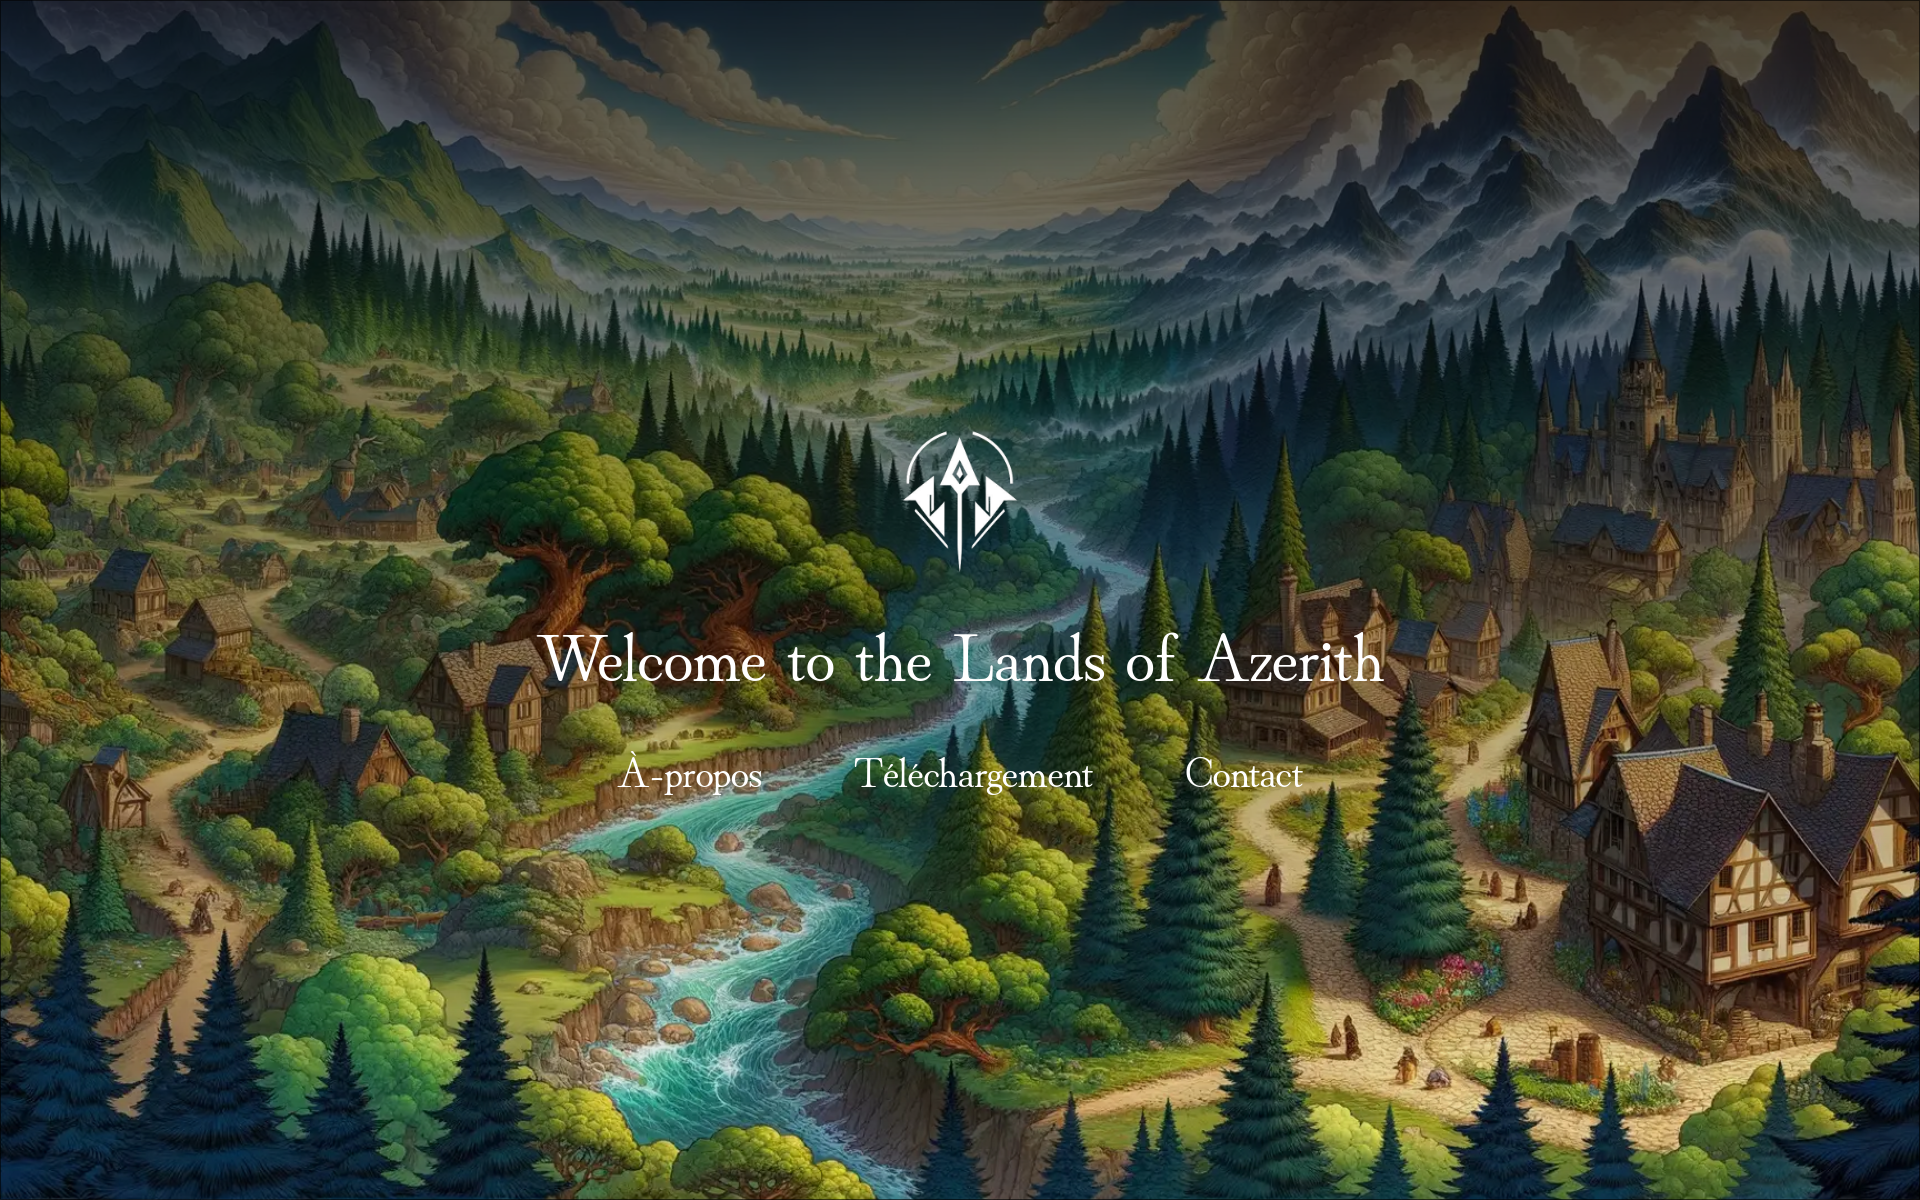
\includegraphics[width=0.8\textwidth]{assets/website1.png}
    \caption{Page d'accueil du site web, elle représente bien la simplicité voulu pour le site web.}
    \label{fig:website1}
\end{figure}

Comme le montre la Figure \ref*{fig:website1}, le site web est simple et épuré.
Il est composé d'une seule page, laissant l'utilisateur scroller pour découvrir les différentes sections.
Elle possède un menu de navigation qui permet de se rendre directement aux sections les plus importantes du site web, et un pied de page avec des liens vers les réseaux sociaux et le dépôt de code source du jeu.
Les différentes sections sont les suivantes :

- "À propos", cette partie présente le jeu, son style et le concept associé

- "Téléchargement", pour télécharger le jeu pour les différentes plateformes

- "Contact", pour contacter l'équipe de développement en redirigeant l'utilisateur vers une adresse mail ou le dépôt GitHub du projet

\subsubsection{Responsive design}

La plus importante amélioration du site web depuis la dernière soutenance est l'ajout du responsive design.
Le site web est maintenant compatible avec les appareils mobiles, et s'adapte automatiquement à la taille de l'écran de l'utilisateur.
Aujourd'hui, la majorité des utilisateurs naviguent sur internet depuis leur smartphone, il est donc essentiel que le site web soit compatible avec ces appareils.

\begin{figure}[H]
    \centering
    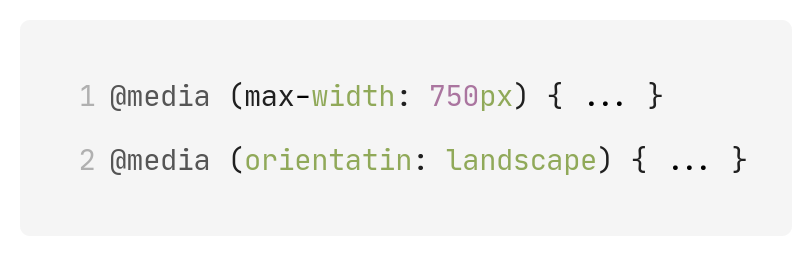
\includegraphics[width=0.6\textwidth]{assets/website2.png}
    \caption{Exemple de \textit{media queries} en CSS.}
    \label{fig:website2}
\end{figure}

Pour réaliser cette amélioration, nous avons utilisé les \textit{media queries} de CSS pour adapter le site web à différentes tailles d'écran.
La Figure \ref*{fig:website2} montre un exemple utilisant cette fonctionnalités du langage CSS.
La première ligne définit le style lorsque la largeur de l'écran est inférieure à 750 pixels, tandis que la deuxième ligne définit le style pour les orientations paysage.
